\documentclass[12pt,a4paper]{article}

\usepackage[utf8]{inputenc} % un package
\usepackage[T1]{fontenc}      % un second package
\usepackage[francais]{babel}  % un troisième package

\usepackage{doi,fullpage,amsmath,charter}
\usepackage{color}
\usepackage{listings}
\usepackage{latexsym}
\usepackage{graphicx}

\title{Préparation au stage recherche \\ Formalisation en TLA+ de programmes parallèles avec\\ modèles mémoire faibles}
\author{Joris RUBAGOTTI}
\date{Avril 2015}
\begin{document}
\maketitle

\section{Présentation du sujet de stage}

\subsection{Présentation grand public}

De nombreuses optimisations reposaient sur le fait que les processeurs possédaient un seul cœur et n'étaient pas observable par les utilisateurs. Aujourd'hui, la majorité des processeurs possèdent au moins deux cœurs. L'utilisateur de la machine peut observer les optimisations et agir sur celles-ci si celui-ci programme de manière à exploiter tous les cœurs ensembles. Mais cette évolution de nos machines apporte une plus grande difficulté à comprendre le fonctionnement de nos processeurs, particulièrement le comportement de la mémoire.

Pour définir le comportement de la mémoire, on a recours aux modèles mémoire. Un modèle mémoire intuitif utilisé dans la programmation parallèle est la consistance séquentielle. On imagine deux programmes que l'on souhaite exécuter en parallèle. Chaque programme est une suite d'instructions. L'exécution en parallèle de ces programmes consiste à entrelacer les instructions de ces deux programmes lors de l'exécution si celle-ci respecte un modèle mémoire séquentiellement consistant. Afin de mieux comprendre ce type de comportement, voici un petit exemple : prenons deux variables $x$ et $y$ ayant pour valeur initiale 0 et deux registres d'un processeur $r_i$ avec $i$ étant le numéro de cœurs auxquels appartient le registre ainsi que le programme suivant suivi des résultats pouvant être obtenu avec un modèle mémoire séquentiellement consistant :
\clearpage
\[
\begin{array}{c||c}
  \begin{array}{l}
    \textcolor[rgb]{0,0,1}{\text{C\oe{}ur 1}} \\
    \textcolor[rgb]{0,0,1}{\mathtt{x = 1;}} \\
    \textcolor[rgb]{0,0,1}{\mathtt{r_0 = y;}} \\
  \end{array} &
  \begin{array}{l}
    \textcolor[rgb]{1,0,0}{\text{C\oe{}ur 2}} \\
    \textcolor[rgb]{1,0,0}{\mathtt{y = 1;}} \\
    \textcolor[rgb]{1,0,0}{\mathtt{r_1 = x;}} \\
  \end{array}
\end{array}
\]
\[
\begin{array}{c||c||c}
  \begin{array}{l}
    \text{Resultat 1} \\
    \textcolor[rgb]{0,0,1}{\mathtt{x = 1;}} \\
    \textcolor[rgb]{0,0,1}{\mathtt{r_0 = y;}} \\
    \textcolor[rgb]{1,0,0}{\mathtt{y = 1;}} \\
    \textcolor[rgb]{1,0,0}{\mathtt{r_1 = x;}} \\
    \mathtt{r_0 = 0, r_1 = 1;} \\
  \end{array} &
  \begin{array}{l}
    \text{Resultat 2} \\
    \textcolor[rgb]{1,0,0}{\mathtt{y = 1;}} \\
    \textcolor[rgb]{1,0,0}{\mathtt{r_1 = x;}} \\
    \textcolor[rgb]{0,0,1}{\mathtt{x = 1;}} \\
    \textcolor[rgb]{0,0,1}{\mathtt{r_0 = y;}} \\
    \mathtt{r_0 = 1, r_1 = 0;} \\
  \end{array} &
    \begin{array}{l}
    \text{Resultat 3} \\
    \textcolor[rgb]{0,0,1}{\mathtt{x = 1;}} \\
    \textcolor[rgb]{1,0,0}{\mathtt{y = 1;}} \\
    \textcolor[rgb]{0,0,1}{\mathtt{r_0 = y;}} \\
    \textcolor[rgb]{1,0,0}{\mathtt{r_1 = x;}} \\
    \mathtt{r_0 = 1, r_1 = 1;} \\
  \end{array} 
\end{array}
\]

Sur la plupart des processeurs actuels, on peut observer un autre résultat possible : $r_0 = 0$ et $r_1 = 0$. En effet, ce résultat peut être obtenu en considérant les cœurs du processeur indépendamment car on observe aucune dépendance dans les instructions de chaque cœurs donc une inversion des instructions est possible pour chaque cœurs cherchant à optimiser leur exécution. Il y a dépendance si dans un cœur, on a comme exemple, une affectation ($x = 1;$) suivi de l'enregistrement de la valeur de cette même variable dans un registre ($r_i = x$). Ce type de comportement nécessite de travailler avec d'autre modèle mémoire possédant moins contraints que la consistance séquentielle. On les appelle modèle mémoire faibles \cite{Adve:1996:SMC:619013.620590}. 

Un modèle mémoire faible possède une propriété fondamentale : si aucune exécution séquentiellement consistante d'un programme parallèle ne contient de data race, c'est à dire deux accès concurrents à la même adresse mémoire dont l'une est une écriture (exemple : $x = 1;$ est une écriture), alors toutes les exécutions de ce programme seront séquentiellement consistantes \cite{Saraswat:2007:TMM:1229428.1229469}.
Si la condition précédente est suffisante, elle n'est pas nécessaire. En effet il existe des conditions plus faible que la data race freeness (DRF), c'est à dire une exécution sans data race, qui permettent d'assurer le comportement séquentiellement consistant d'un programme. De nombreux travaux sur la vérification de ce type de programme tenant compte du modèle mémoire faible ont été réalisés.

C'est dans ce contexte que mon stage, proposé par Frédéric LOULERGUE, professeur au LIFO\footnotemark[1] à l'Université d'Orléans, intervient. Je devrai comprendre et employer le langage TLA+ \cite{Lamport:2002:SST:579617} et l'environnement associé à ce langage afin de formaliser un ou plusieurs modèles mémoire faibles et ensuite utiliser cette formalisation pour prouver la correction de programmes parallèles dans le contexte d'un modèle mémoire faible. 
  
\subsection{Présentation Master Informatique}

De nombreuses optimisations reposaient sur le fait que les processeurs possédaient un seul cœur et n'étaient pas observables par les utilisateurs.
Aujourd'hui, les processeurs multi-cœurs et la programmation parallèle sont courants. Ces optimisations deviennent visibles pour l'utilisateur, et rendent la sémantique des processeurs complexes, particulièrement sur le comportement de la mémoire.

Un modèle mémoire intuitif utilisé dans la programmation parallèle est la consistance séquentielle. Les exécutions de deux programmes mis en parallèle sont les entrelacements des exécutions des deux programmes considérés séparément. Par exemple, on a deux variables x et y ayant pour valeur initiale 0 et deux registres d'un processeur $r_i$ ainsi que le programme suivant :
\[
\begin{array}{c||c}
  \begin{array}{l}
    \textcolor[rgb]{0,0,1}{\text{C\oe{}ur 1}} \\
    \textcolor[rgb]{0,0,1}{\mathtt{x = 1;}} \\
    \textcolor[rgb]{0,0,1}{\mathtt{r_0 = y;}} \\
  \end{array} &
  \begin{array}{l}
    \textcolor[rgb]{1,0,0}{\text{C\oe{}ur 2}} \\
    \textcolor[rgb]{1,0,0}{\mathtt{y = 1;}} \\
    \textcolor[rgb]{1,0,0}{\mathtt{r_1 = x;}} \\
  \end{array}
\end{array}
\]
On déduit les résultats suivants avec un modèle mémoire séquentiellement consistant :
\begin{itemize}
	\item $r_0 = 0$ et $r_1 = 1$
	\item $r_0 = 1$ et $r_1 = 0$
	\item $r_0 = 1$ et $r_1 = 1$
\end{itemize} 
Sur la plupart des processeurs actuels, on peut observer aussi le résultat $r_0 = 0$ et $r_1 = 0$. En effet, ce résultat peut être obtenu en considérant les cœurs du processeur indépendamment car on observe aucune dépendance dans les instructions de chaque cœurs donc une inversion des instructions est possible pour chaque cœurs. Ce type de comportement nécessite l'utilisation de modèle mémoire moins contraint que la consistance séquentielle. On les appelle modèle mémoire faibles \cite{Adve:1996:SMC:619013.620590}. 

Un modèle mémoire faible possède une propriété fondamentale. Si aucune exécution séquentiellement consistante d'un programme parallèle ne contient de data race, c'est à dire deux accès concurrent  à la même adresse mémoire dont l'une est une écriture, alors toutes les exécutions de ce programme seront séquentiellement consistantes \cite{Saraswat:2007:TMM:1229428.1229469}.
Si la condition précédente est suffisante, elle n'est pas nécessaire. En effet il existe des conditions plus faible que la data race freeness (DRF), qui permettent d'assurer le comportement séquentiellement consistant d'un programme. De nombreux travaux sur la vérification de ce type de programmes tenant compte du modèle mémoire faible ont été réalisés.

C'est dans ce contexte que mon stage, proposé par Frédéric LOULERGUE, professeur au LIFO\footnotemark[1] à l'Université d'Orléans, intervient. Je devrai comprendre et employer le langage TLA+ \cite{Lamport:2002:SST:579617} et l'environnement associé à ce langage afin de formaliser un ou plusieurs modèles mémoire faibles et ensuite utiliser cette formalisation pour prouver la correction de programmes parallèles dans le contexte d'un modèle mémoire faible. 

\subsection{Présentation chercheur}
De nombreuses optimisations reposaient sur le fait que les processeurs possédaient un seul cœur et n'étaient pas observable par les utilisateurs.
Aujourd'hui, les processeurs multi-cœurs et la programmation parallèle sont courants. Ces optimisations deviennent visibles pour l'utilisateur, et rendent la sémantique des processeurs complexes, particulièrement sur le comportement de la mémoire.

Un modèle mémoire intuitif utilisé dans la programmation parallèle est la consistance séquentielle. Les exécutions de deux programmes mis en parallèle sont les entrelacements des exécutions des deux programmes considérés séparément.
 
Ce modèle mémoire n'est pas suffisant pour expliquer le comportement des processeurs actuels. En effet, des résultats ne pouvant pas apparaitre dans le contexte de consistance séquentielle sont pourtant présents. Pour comprendre ce type de comportement, il est nécessaire d'utiliser des modèles mémoire faibles \cite{Adve:1996:SMC:619013.620590} moins contraignant. 

Une propriété fondamentale des modèles mémoire faibles consiste en si aucune exécution séquentiellement consistante d'un programme parallèle ne contient de data race, alors toutes les exécutions de ce programme seront séquentiellement consistantes \cite{Saraswat:2007:TMM:1229428.1229469}.
Si la condition précédente est suffisante, elle n'est pas nécessaire. En effet il existe des conditions plus faible que la data race freeness (DRF), qui permettent d'assurer le comportement séquentiellement consistant d'un programme. De nombreux travaux sur la vérification de ce type de programmes tenant compte du modèle mémoire faible ont été réalisés.

C'est dans ce contexte que mon stage, proposé par Frédéric LOULERGUE, professeur au LIFO\footnotemark[1] à l'Université d'Orléans, intervient. Je devrai comprendre et employer le langage TLA+ \cite{Lamport:2002:SST:579617} et l'environnement associé à ce langage afin de formaliser un ou plusieurs modèles mémoire faibles et ensuite utiliser cette formalisation pour prouver la correction de programmes parallèles dans le contexte d'un modèle mémoire faible. 
 
\footnotetext[1]{Laboratoire d'Informatique Fondamentale d'Orléans} 

\section{Les modèles mémoire faibles}

\subsection{Contexte}

Avant d'expliquer un peu plus en détail les modèles mémoire faibles, il est nécessaire de comprendre les raisons de leur utilisation. Avant le développement des processeurs ayant plusieurs cœurs, les concepteurs de micro-processeur recherchaient les meilleurs performances pour les processeurs avec un seul cœur. Pour ce faire, ils cherchaient principalement à croitre la fréquence ou à optimiser les exécutions des instructions au sein d'un cœur ressemblant à du parallélisme "interne" au cœur. Mais aujourd'hui, il devient difficile de croitre la fréquence d'un processeur pour diverses raisons technique comme la dissipation thermique. Pour compenser cela, les concepteurs de processeurs ont multipliés le nombre de cœurs sur les processeurs dans le but d'exécuter des morceaux d'un programme simultanément.

Cette nouvelle forme d'architecture pose des problèmes d'adaptation. En effet, malgré de nombreuses études théoriques, la parallélisation reste complexe. Plusieurs causes de cette difficulté existent :
\begin{itemize}
	\item Les algorithmes ne sont pas tous adaptés au contexte parallèle
	\item Les optimisations pour un cœur cité plus haut sont la source de conflit avec le parallélisme obtenu avec plusieurs cœurs. 
\end{itemize}
L'étude de ces problèmes et de leur résolution à donner naissance aux modèles mémoire faibles.

Un modèle mémoire ressemble au méthode de description d'un langage de programmation par des chercheurs en programmation d'un point de vu sémantique, c'est à dire les résultats que l'on peut obtenir avec des bouts de code du langage. Un modèle mémoire intuitif, dans le contexte du parallélisme, est la consistance séquentielle. Ce modèle mémoire est énoncé par Leslie Lamport en 1979 posant les bases de la programmation parallèle. Ce modèle définit que toutes exécutions du programme multi cœurs se faisait toujours en exécutant les instructions de chaque thread une par une dans l'ordre du programme. Le modèle  consistance séquentielle est modèle très appliquer les développer principalement. Quand celui-ci développe son programme sur plusieurs cœurs, il a tendance à suivre ce modèle. Les modèles mémoire des processeurs actuels sont plus faible que le modèle de consistance séquentielle, comme ceux-ci apportent moins de garanties. En effet, toute séquence d'exécution valide dans le modèle séquentiel est également valide dans un modèle plus faible.

Une autre raison de l'utilisation des modèles mémoire faibles est la recherche de meilleur performance. En effet, afin d'éviter les data race dans les programmes, des locks sont utilisés pour construire des sections sûr lors de l'exécution. Data race est le nom donné à un accès concurrent, sur même zone mémoire, par deux cœurs différents dont l'un de ces accès est une écriture. Le problème de l'utilisation de ces locks, l'exécution n'est plus parallèle, lorsque d'autres écritures par d'autre cœurs sont nécessaires, durant cette section d'où une perte de performance. L'utilisation des modèles mémoire faibles permettent de vérifier la validité des résultats de certains programmes ayant des data race mais respectant le modèle de la consistance séquentielle donc l'absence d'utilisation de locks dans ces cas permettent un gain de performance.  

\subsection{Introduction au modèle mémoire des processeurs x86}
 
Dans cette partie, on introduit un modèle mémoire faible x86-TSO utilisé pour les processeurs x86. Pour la spécification de ce modèle, on reprend la spécification proposée dans l'article \cite{Sewell:2010:XRU:1785414.1785443}. Cette spécification est née de la recherche de compréhension des processeurs x86. En effet, la documentation fournit par Intel propose que des proses informelles sur le sujet. L'analyse de ces proses montre des erreurs lors de test de validité du modèle (nommé aussi litmus test). Afin de remédier à ces manques, le modèle mémoire x86-TSO est proposé pour mieux comprendre certains résultats. Il est défini mathématiquement en deux styles :
\begin{itemize}
	\item Une machine abstraite avec des buffers de stockage explicite.
	\item Un modèle axiomatique qui définit la validité des exécutions selon l'ordre dans la mémoire. 
\end{itemize}
La machine abstraite transmet l'idée au niveau du programmeur sur x86-TSO. Le modèle axiomatique apporte un raisonnement par contrainte sur les exemples de programmes tests que l'on verra un peu plus loin. Il est important de signaler les instructions atomiques proposé dans l'architecture x86 : l'une peu ajouter un LOCK prefix sur plusieurs instructions lecture-modification-écritures (ADD, INC, etc.), et l'instruction XCHG est implicitement LOCK'd. Il y a trois barrière pour la mémoire : MFENCE, SFENCE et LFENCE.

\subsubsection*{Machine abstraite}

\begin{figure}[ht]
	\begin{center}
		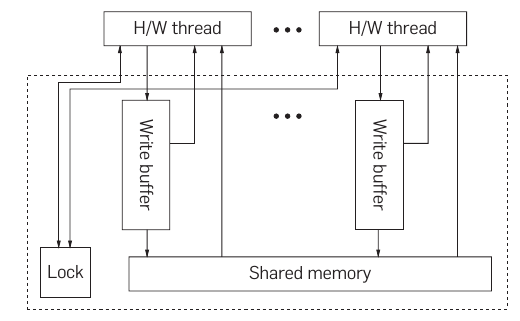
\includegraphics[scale=0.8]{mach_abst.png}
		\caption{x86-TSO : machine abstraite}	
	\end{center}
\end{figure}

Pour comprendre le fonctionnement de la machine abstraite, plusieurs informations sont nécessaires. Le comportement du stockage suit les points suivants :
\begin{itemize}
	\item Le buffer de stockage est une FIFO (First In First Out) et un thread en lecture doit lire l'écriture la plus récente du buffer, si il y en a une, à cette adresse; Autrement les lectures se font au niveau de la mémoire partagée.
	\item L'instruction MFENCE vide le buffer de stockage du thread.
	\item Pour exécuter une instruction LOCK'd, un thread doit obtenir le lock global dans un premier temps. A la fin de l'instruction, il vide le buffer de stockage et libère le lock. Tant qu'un lock est tenu par un thread, les autres threads ne peuvent pas lire. 
\end{itemize}
Si on veux être plus précis, les possibles interactions entre les threads et le sous-système de stockage sont décrites par les évènements suivants :

\begin{itemize}
	\item $W_p[a]=u$, pour une valeur écrit $u$ à l'adresse $a$ par le thread $p$	
	\item $R_p[a]=u$, pour une valeur lu $u$ à l'adresse $a$ par le thread $p$
	\item $F_p$ , pour une barrière de mémoire MFENCE par le thread $p$
	\item $L_p$ , au début de l'instruction LOCK'd par le thread $p$
	\item $U_p$ , à la fin de l'instruction LOCK'd par le thread $p$
	\item $\tau_p$ , pour une action interne du sous-système de stockage, propage l'écriture du buffer de stockage de $p$ vers la mémoire partagée.
\end{itemize}

Par exemple, le thread $p$ exécute l'instruction INC[56] (ajoute 1 a la valeur à l adresse 56), et le buffer de stockage de $p$ contient une seule écriture à l'adresse 56 de valeur 0. Pour une seule exécution, on a des évènements de lecture et d'écriture, $R_p[56] = 0$ et $W_p[56] = 1$, suivi de 2 évènements $\tau_p$ pour propager les deux écritures vers la mémoire partagée.
Ensuite on donne la spécification du comportement du sous-système de stockage avec les règles suivantes :
\begin{enumerate}
	\item $R_p[a] = u$ : $p$ peut lire $u$ de la mémoire à l'adresse $a$ si $p$ n'est pas bloqué, si aucune écriture de $a$ soit présente dans le buffer de $p$ et la mémoire contient déjà $v$ à l'adresse $a$
	\item $R_p[a] = u$ : $p$ peut lire $u$ du buffer de l'adresse $a$ si $p$ n'est pas bloqué et a $u$ comme une nouvelle écriture vers $a$ dans son buffer.
	\item $W_p[a] = u$ : $p$ peut écrire $u$ dans son buffer pour l'adresse $a$ quand il le souhaite.
	\item $\tau_p$ : si $p$ n'est pas bloqué, il peut sortir la plus vielle valeur d'écriture de son buffer et placer la valeur en mémoire à l'adresse donnée, sans coordination avec les autres cœurs.
	\item $F_p$ : si le buffer de $p$ est vide, il peut alors exécuter MFENCE.
	\item $L_p$ : si lock n'est pas en attente, l'instruction LOCK'd peut commencer.
	\item $U_p$ : si $p$ a le lock, et son buffer est vide, il peut mettre fin à l'instruction LOCK'd.
\end{enumerate}

Voilà pour les règles pour cette spécification. Maintenant il est intéressant de voir si c'est spécification réussi quelques tests.

\subsubsection*{Litmus tests}

Il s'agit de tests utilisés afin de valider le modèle mémoire x86-TSO. Ces tests proviennent de la documentation d'Intel sur leur processeur.

\paragraph{EXEMPLE 1 : STORES ARE NOT REORDERED WITH OTHER STORES.}

	\begin{center}
		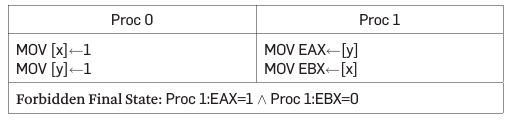
\includegraphics[scale=0.9]{exemple1.png}
	\end{center}

Ce test implique que les écritures par le Proc 0 sont vues dans l'ordre par les lectures du Proc 1 qui s exécute aussi dans l'ordre. x86-TSO interdit l'état final parce que le buffer de Proc 0 est une FIFO et Proc 0 communique avec Proc 1 via seulement la mémoire partagée.

\paragraph{EXEMPLE 2 : STORES ARE NOT REORDERED WITH OLDER LOADS.}
  
	\begin{center}
		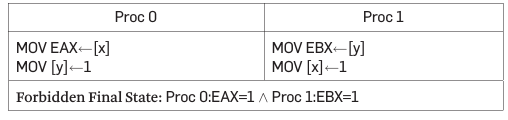
\includegraphics[scale=0.9]{exemple2.png}
    \end{center}

x86-TSO interdit l'état final parce que la lecture n'est jamais retardée.
Beaucoup d'autre tests sont possibles pour vérifier la cohérence du modèle mais ils seraient trop long dans aborder plus dans ce document. Cette spécification n'est pas codé par nos main à l'heure actuelle. Mais le projet de ce stage est de formaliser en TLA+ la spécification précédente et d'effectuer des tests plus précis sur le modèle.

\section{Le langage TLA+}

\subsection{Introduction au langage}

TLA+ est un langage de spécification et de preuve basé sur la logique temporelle. En utilisant la logique du premier ordre et la théorie des ensembles, on décrit un ensemble d'états et les possibles transitions entre ces états. Les systèmes sont spécifiés en TLA+ comme formules Temporal Logic
of Actions TLA, une variante de la logique temporelle linéaire introduite par Lamport.

Pour mieux comprendre le langage, commençons par construire un premier système. Prenons en exemple une horloge digitale qui affiche seulement les heures que l'on nommera HourClock. Le comportement d'une horloge est la séquence d'états, où $[hr = 11]$ est un état dans lequel $ hr $ est de valeur 11.
$$ [hr = 11] \rightarrow [hr = 12] \rightarrow [hr = 1] \rightarrow [hr = 2] \rightarrow ...$$
Une paire successive d'états, tel que $[hr = 1] \rightarrow [hr = 2]$, est nommé un pas.
Pour spécifier l'horloge, on décrit tous les comportements possibles. Dans notre cas, il faut un prédicat initial pour spécifier les choix possibles de valeur pour $hr$ et la relation pas suivant qui spécifie comment la valeur $hr$ peut évoluer à chaque pas.
Le prédicat initial est nommé $HCini$ et ce prédicat affirme que la valeur initial de $hr$ est comprise entre 1 et 12. On obtient ainsi la définition suivante :

$$ HCini == hr \in \{1,...,12\}$$

Le symbole "==" signifie est défini comme égale à ... 
La relation de transition entre les pas $HCnxt$ est une formule exprimant la relation entre la valeur $hr$ dans l'ancien état et $hr'$ ($'$ prononcé prime) dans le état suivant. On définit $HCnxt$ en utilisant la construction if/then/else avec la relation suivante :   

$$ HCext == hr' = \text{if } hr \neq 12 \text{ then } hr + 1 \text{ else } 1 $$

Le type de formule utilisant la notation prime $'$ est nommé action. Un pas satisfait l'action $HCnext$ est appelé un $HCnxt$ pas.
Pour finir, on souhaite que notre spécification corresponde à une seule formule et non une paire de formules. La formule doit affirmer le comportement suivant :
\begin{enumerate}
	\item L'état initial satisfait $HCini$
	\item Chaque pas satisfait $HCnxt$
\end{enumerate}
Pour le premier cas, on l'exprime comme la formule $HCini$. Pour le deuxième cas, on utilise un opérateur de logique temporelle $\Box$ (prononcé box). La formule temporelle $\Box F$ affirme que la formule est toujours vraie. On ajoute à la spécification que la valeur $hr$ peut rester identique entre deux pas avec la notation $\Box [HCnxt]_{hr}$ pouvant être notée $\Box (HCnxt \lor (hr' = hr ))$. Donc on obtient comme formule, nommée $HC$, suivante :

$$ HC == HCini  \land  \Box [HCnxt]_{hr} $$

Pour obtenir la spécification en TLA+, on doit écrire la spécification en ASCII. La conversion de certains symboles se font de la manière suivante :

\begin{itemize}
	\item $\in$ se traduit par $\backslash in$
	\item $\Box$ par []
	\item $\neq$ par \#
	\item $\land$ et $\lor$ par $/ \backslash$ $\backslash /$ 
\end{itemize}

On obtient donc la spécification en TLA+ suivante

\begin{figure}[ht]
\begin{lstlisting}[frame=single, basicstyle=\footnotesize]
----------------------------- MODULE HourClock ----------------------------
EXTENDS Naturals
VARIABLE hr
---------------------------------------------------------------------------
HCini == hr \in (1 .. 12)
HCnxt == hr' = IF hr # 12 THEN hr + 1 ELSE 1
HC == HCini /\ [][HCnxt]_hr
---------------------------------------------------------------------------
THEOREM HC => []HCini
===========================================================================

\end{lstlisting}
\caption{La spécification de HourClock ASCII versions}
\end{figure}

Les lignes -------- sont purement esthétiques. Elles servent à séparer les différentes déclarations selon leurs significations. Comme première ligne, on a le nom du module précédé du mot clef MODULE.
Ensuite on a une phase "d'initialisation" où on déclare les variables de notre spécification avec le mot clef VARIABLE suivi des noms de ceux-ci. Pour pouvoir employer des opérateurs usuelles de mathématique, il est nécessaire de les importer. Dans notre spécification, on utilise des opérateurs sur des nombres naturelles donc on importe avec le mot clef EXTENDS le module Naturals.
Dans la partie suivante, on ajoute nos différents prédicats que l'on a définis précédemment.
En dernière partie, on a la déclaration suivante :
$$ \text{THEOREM } HC \Rightarrow \Box HCini$$
Il s'agit de la déclaration des théorèmes. Elle affirme que la formule $HC \Rightarrow \Box HCini$ est vraie dans le contexte de la déclaration. Plus précisément il affirme que la formule suit logiquement les définitions du module, les définitions dans le module Naturals et les règles de TLA+. Si la formule était fausse , alors le module serait incorrect.
Voilà un premier module TLA+. Il ne s'agit pas de la seule spécification d'une horloge avec seulement la gestion des heures possible. D'autres spécifications sont possibles tel que l'utilisation du modulo pour réaliser la relation $HCnxt$ :

$$ HCnxt2 == hr' = (hr \% 12) + 1 $$
Le symbole $ \% $ correspond à l'opérateur modulo dans le module Naturals. 

\subsection{An Asynchronous Interface : un autre exemple}

On formalise maintenant l'interface pour transmettre des données entre des appareils asynchrones.

\begin{figure}[ht]
	\begin{center}
		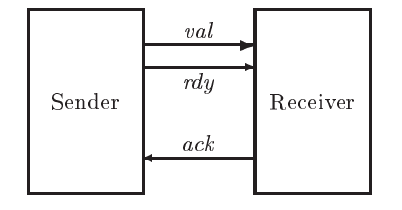
\includegraphics[scale=0.7]{schema_async.png}
		\caption{Schéma du système}	
	\end{center}
\end{figure}

La donnée est envoyée via la variable $val$ et les variables $rdy$ et $ack$ sont utilisées pour la synchronisation.

\begin{figure}[ht]
	\begin{center}
		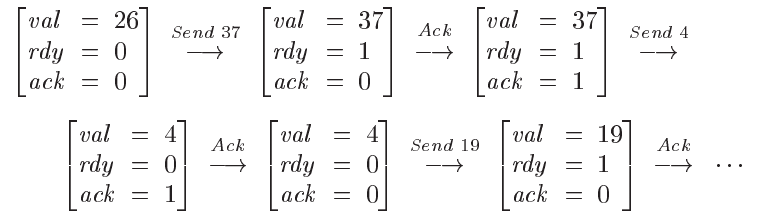
\includegraphics[scale=0.7]{exemple_async.png}
		\caption{Exemple d'exécution}	
	\end{center}
\end{figure}

Il faut bien comprendre qu'une spécification est une abstraction. Elle décrit la plupart des aspects d'un système et en ignore d'autres. Par exemple, dans la spécification présente,  on ignore un facteur temps présent entre les transitions dans la réalité. Dans notre contexte, on considère les transitions entre les états prennent un temps nul.

C'est en prenons en compte l'idée précédente que l'on obtient la spécification TLA+ suivante :

\begin{figure}[ht]
\begin{lstlisting}[frame=single, basicstyle=\footnotesize]
---------------------- MODULE AsynchInterface -----------------------------
EXTENDS Naturals
CONSTANT Data
VARIABLE chan
TypeInvariant == chan \in [val:Data, rdy:{0,1}, ack:{0,1}]
---------------------------------------------------------------------------
Init == /\ TypeInvariant
        /\ chan.ack = chan.rdy
        
Send(d) == /\ chan.rdy = chan.ack
           /\ chan' = [chan EXCEPT !.val = d, !.rdy = 1 -@]
           
Rcv == /\ chan.rdy # chan.ack
       /\ chan' = [chan EXCEPT !.ack = 1 - @]

Next == (\E d \in Data : Send(d)) \/ Rcv
Spec == Init /\ [][Next]_chan
---------------------------------------------------------------------------
THEOREM Spec => []TypeInvariant       

===========================================================================
\end{lstlisting}
\caption{La spécification de AsynchInterface ASCII versions}
\end{figure}

Cette spécification introduit de nouveaux concepts disponible avec le langage TLA+. Dans la première partie, on utilise EXTENDS pour les opérateurs des nombres naturels. Ensuite on introduit le mot clef CONSTANT. CONSTANT introduit un nom symbolique. $Data$ est un paramètre de la spécification.
Ensuite on déclare la variable $chan$. Une dernière déclaration est TypeInvariant qui est un prédicat indiquant quelles valeurs peuvent être utilisées selon le comportement satisfaisant la spécification. Dans ce cas si, chan est un objet nommé record pour TLA+ se traduisant par un tuple en mathématique. Le champ $val$ peut prendre n'importe quelles valeurs données par le paramètre $Data$. Les champs $val$ et $rdy$ peuvent égales à 1 ou 0 seulement.

Dans la seconde partie du module, on a les différents prédicats. L'état initial $Init$ donne les conditions d'initialisation, c'est à dire le respect du prédicat $typeInvariant$ et de l'égalité entre le champ $ack$ et $rdy$ du record $chan$. $Send(d)$ peut prendre en paramètre une valeur nommée $d$ respectant $Data$. Le prédicat est vrai si $ack$ et $rdy$ de $chan$ sont égaux. Pour le pas suivant, on a une transition entre les états avec $chan'$. $chan'$ prend les mêmes valeurs que $chan$ exceptées (via le mot clef EXCEPT) du champs $val$ prenant la valeur $d$ et le champs $rdy$ qui prend la valeur $1 - chan.rdy$ avec $chan.rdy$ symbolisée par @ dans ce prédicat.
Ensuite on a le prédicat $Rcv$ testant si $ack$ et $rdy$ sont bien différentes et effectue une transition de la valeur $chan$.
Le prédicat $Next$ vérifie $Send(d)$ ou $Rcv$ en testant si $d$ est une valeur dans Data. Pour finir on a la spécification avec le prédicat $Spec$ vérifiant si $Init$ est vrai et que $Next$ soit toujours vrai ou si $chan$ reste inchangée.

En dernière partie, on a le théorème affirmant que le prédicat $TypeInvariant$ est toujours vrai dans cette spécification.

TLA+ possède aussi d'autres outils permettant diverses vérifications d'une spécification. Pour le moment n'ayant pas exploité ces outils moi-même mais leur utilisation est nécessaire pour la réussite du stage, il m'est difficile d'expliquer proprement leur fonctionnant. Un premier outil est nommé TLC model checker. Un autre outils pouvant être utilisé au sujet est TLA proof system. il permet d'écrire des preuves structurées hiérarchiquement et via un gestionnaire de preuve permettant de vérifier ces preuves.  

\section{Conclusion}

Si l'on doit résumer cette première partie du stage, on possède une première spécification d'un modèle mémoire faible avec le x86-TSO. On commence à obtenir un début de maitrise du langage TLA+ et de ces outils mais beaucoup de travail reste à faire si je veux pouvoir réaliser une bonne spécification du modèle x86-TSO en TLA+. Si les premiers tests donnent de bons résultats, il sera intéressant d'étudier les modèles mémoire faibles de différentes architectures de processeur tel que ARM ou PowerPC.

\clearpage

\bibliographystyle{ieeetr}
\bibliography{biblio}
\nocite{Alglave:2009:SPA:1481839.1481842, Owens:2010:RIC:1883978.1884011, PETRI, Saraswat:2007:TMM:1229428.1229469, Sewell:2010:XRU:1785414.1785443, Turon:2014:GNW:2714064.2660243, Boehm:2011:YDK:2076796.2088916}
\end{document}